%; whizzy chapter
% -initex iniptex -latex platex -format platex -bibtex jbibtex -fmt fmt
% 以上 whizzytex を使用する場合の設定。


%     Tokyo Debian Meeting resources
%     Copyright (C) 2008 Junichi Uekawa
%     Copyright (C) 2008 Nobuhiro Iwamatsu

%     This program is free software; you can redistribute it and/or modify
%     it under the terms of the GNU General Public License as published by
%     the Free Software Foundation; either version 2 of the License, or
%     (at your option) any later version.

%     This program is distributed in the hope that it will be useful,
%     but WITHOUT ANY WARRANTY; without even the implied warranty of
%     MERCHANTABILITY or FITNESS FOR A PARTICULAR PURPOSE.  See the
%     GNU General Public License for more details.

%     You should have received a copy of the GNU General Public License
%     along with this program; if not, write to the Free Software
%     Foundation, Inc., 51 Franklin St, Fifth Floor, Boston, MA  02110-1301 USA

%  preview (shell-command (concat "evince " (replace-regexp-in-string "tex$" "pdf"(buffer-file-name)) "&"))
% 画像ファイルを処理するためにはebbを利用してboundingboxを作成。
%(shell-command "cd image200804; ebb *.png")

%%ここからヘッダ開始。

\documentclass[mingoth,a4paper]{jsarticle}
\usepackage{monthlyreport}

% 日付を定義する、毎月変わります。
\newcommand{\debmtgyear}{2008}
\newcommand{\debmtgmonth}{8}
\newcommand{\debmtgdate}{11}
\newcommand{\debmtgnumber}{43}

\begin{document}

\begin{titlepage}
\thispagestyle{empty}

% タイトルページ:編集必要な部分は最初のマクロに飛ばすこと

\vspace*{-2cm}
第\debmtgnumber{}回 東京エリア Debian 勉強会資料

\hspace*{-2.4cm}
\includegraphics[width=210mm]{image200801/2008title.eps}\\
\hfill{}\debmtgyear{}年\debmtgmonth{}月\debmtgdate{}日

\end{titlepage}

\dancersection{Introduction}{上川 純一}
 
 今月のDebian勉強会へようこそ。これからDebianの世界にあしを踏み入れると
 いう方も、すでにどっぷりとつかっているという方も、月に一回Debianについ
 て語りませんか?

 Debian勉強会の目的は下記です。

\begin{itemize}
 \item \underline{Debian Developer} (開発者)の育成。
 \item 日本語での「\underline{開発に関する情報}」を整理してまとめ、アップデートする。
 \item \underline{場}の提供。
 \begin{itemize}
  \item 普段ばらばらな場所にいる人々が face-to-face で出会える場を提供
	する。
  \item Debian のためになることを語る場を提供する。
  \item Debianについて語る場を提供する。
 \end{itemize}
\end{itemize}		

 Debianの勉強会ということで究極的には参加者全員がDebian Packageをがりがり
 と作るスーパーハッカーになった姿を妄想しています。情報の共有・活用を通し
 て Debianの今後の能動的な展開への土台として、「場」としての空間を提供す
 るのが目的です。

以上を目的とした、2008 年アジェンダです:
\begin{enumerate}
 \item 新年会「気合を入れる」
 \item Open Source Conference Tokyo (3/1)
 \item データだけのパッケージを作成してみる、
       ライセンスの考え方 (David Smith)
 \item バイナリ一つのパッケージを作成してみる (吉田@板橋)\\
       バージョン管理ツールを使いDebianパッケージを管理する(git)\\
       アップストリームの扱い(svn/git/cvs)(岩松 信洋さん)
 \item バイナリの分けたパッケージの作成。(前田さん)\\
       バイナリの分け方の考え方、アップグレードなどの運用とか。
 \item パッケージ作成(dpatch/debhelperで作成するパッケージ)(小林儀匡さん)\\
       OSC 2008 Hokkaido
 \item パッケージ作成(kernel patch、kernel module)(岩松 信洋)
 \item Debconf アルゼンチン、Debian 温泉 \\
       コミックマーケット74
 \item Open Source Conference Tokyo/Fall、
       デーモン系のパッケージの作成、latex、 emacs-lisp、フォントパッケージ
 \item パッケージの cross-compile の方法、amd64 上で i386 のパッケージと
       か、OSC-Fall報告会、Debconf報告会
 \item 国際化 po-debconf / po化 / DDTP
 \item 忘年会
\end{enumerate}


\newpage

\begin{minipage}[b]{0.2\hsize}
 \definecolor{titleback}{gray}{0.9}
 \colorbox{titleback}{\rotatebox{90}{\fontsize{80}{80} {\gt デビアン勉強会} }}
\end{minipage}
\begin{minipage}[b]{0.8\hsize}
\hrule
\vspace{2mm}
\hrule
\tableofcontents
\vspace{2mm}
\hrule
\end{minipage}

\dancersection{最近のDebian関連のミーティング報告}{岩松 信洋}
\subsection{東京エリアDebian勉強会42回目報告}

東京エリアDebian勉強会報告。 7月の第42回東京エリアDebian勉強会を実施しました。今回の参加者は あけどさん、前田耕平さん、伊藤弘和さん、鈴木崇文さん、山本浩之さん、山本琢さん、やまねひできさん、おおなみまことさん、たかすぎやすひこさん、本庄さん、日比野啓さん、青木 修さん、藤沢理聡さん、David Smithさん、関根さん、鵜飼文敏さん、岩松 の 17名でした。

まず、クイズを今回も実施しました。 今回は、debian-devel-announce に投稿された内容とDebian Project News から出題しました。3問目ぐらいでみんな不正解になったので、敗者復活をしましたが、皆さんすぐに間違えてしまいました。3階ほど敗者復活してしまいました。みなさん、ちゃんと Debian Project News を読みましょうね。

Linux カーネルパッチパッケージの作成方法について説明しました。かなりニッチなパッケージではありますが、Linux のリリースサイクルとDebianのリリースサイクル、そしてユーザの要望を考えると、必要なパッケージになるということと、あまり使う人がいないパッケージなので、みなさんは興味を持って聞いていました。 dh-make を使ったLinux カーネルパッチパッケージの雛形を作成する方法がサポートされていないのですが、今回の発表による成果物がBTSされたようです。実装されることを期待しましょう。

Linux モジュールパッケージの作成方法について説明しました。パッケージの作成段階と、それによって生成される各ファイルの説明、現時点での問題点について解説し、参加者で対応方法について議論しました。

Debian 温泉について話しました。次回の勉強会開催予定日は Debian15周年。みんなで温泉に入りながらハックしたり、日頃の疲れを癒しませんか、ということで企画している旨を伝えました。10人ほど集まりそうです。

やまねさんが lenny に向けて、現在確認されている日本語での問題について説明しました。また、翻訳の査読が滞っているので査読者を募集しました。"てにおは"のチェックだけでもかなりありがたいので、協力者はdeian-doc ML に入って、チェックをよろしくお願いします。

今後のDebian勉強会と、ユーザと連動した内容をどうするか、ということについてみんなで話し合いました。最近は Debian のパッケージ化、開発者寄りの話になっているので、ユーザ側の意見を取り入れたり、問題を受け入れやすくする場を作るためにどうしたらいいのか、ということを考えました。結果、各言語や、フレームワーク、システムなどをDebianでどのように使っているのか、また使えるのか、実際にやっておられる方に話してもらうとユーザはわかりやすいのではないか、ということになりました。その場でやっていただける方がおられたので、今後の発表に期待しましょう。

今回は宴会は 庵GuRi(あぐり) 5566 にて開催しました。 


\dancersection{Debconf 8}{岩松 信洋}
\label{sec:debconf8}
\index{debconf8}

勉強会として、今回の Debconf 開催地である アルゼンチンからIRCを使って行われました。内容を以下に報告します。

\subsection{当日のアジェンダ}
\begin{enumerate}
\item 22:00-  Debconf 参加者 の 今回の意気込み
\item 22:30-  Debconf 参加者 への Debconf 質問コーナー
\end{enumerate}

\subsection{参加者}
\begin{itemize}
\item debconf側

 上川さん(dancer)

\item 日本側
kmuto, henrich, yamamoto, aya, honjo, risou, mkouhei, ake, iwamatsu
\end{itemize}

\subsection{参加者への質問}
Debconf 参加者への質問ということで、以下の質問があり、参加者から回答を得ることができました。
質問内容 (質問者名) という形式になっています。

\begin{enumerate}
\item 無事にたどりつけましたか (kmuto)

  予約待ちしていたバスが予約できていなかったので、retiro 経由でバス8時間、合計40時間の行程でした。今回しかも、san francisco からの旅程なので、日本からいってたら死ねる (dancerj) 

\item wife様がgeekどもを見て一言 (匿名)

  「ほどほどにね」 

\item 日本からは(そもそも)誰が行っているのですか?(AyaKomuro)

   上川さん夫妻です(奥様可哀想と言う声もあるような…「アルゼンチンに旅行にいく、としか説明していなかった・・・」) 

\item 今回のDebconfで期待しているセミナー/レクチャーは何ですか?(AyaKomuro)

   「基本的に期待していないので、Hacklab にずっといるつもりです。」 

\item Debconf@Argentinaならではのこれは!?を教えてください(AyaKomuro)

  \begin{itemize}
    \item keysigning party に出ないつもりなので個別にkeysigningをする。
    \item qemu maintainer groupに強制収容された、qemubuilder ハックした
    \item あと Don armstrongをつかまえてBTS SOAP のインタフェースのバグを直してもらうかな
  \end{itemize} 
\item 日本で debconf 開いたら来たいよーって人はどのくらいいるのでしょうか? (henrich)
   
  「明日、19:00 からdebconf10会議がある。」 

\item ごはんはおいしいのかな (kmuto)

   「ごはんうまいっす。かなり。いけてる。朝飯からケーキ。牛メインですね。港町なので魚もある。野菜はすくな目かな。パンはそうでもないです。debconf の会場のそとで食事したら多分肉肉してるんだろうけど、ホテルの食事はそうでもないです。」 
\item 日本の Debian 関係者に何か一言ないか。(henrich)

  無回答
\item Lenny で DDTP のエンコードによる文字化け問題は解決の見込みがあるのか (henrich)

  無回答
\item unzip の表示がおかしくなる問題について、Ubuntu のメンテナとの協業で解決してはもらえないのか。大変この問題を憂いている。(henrich)
       
    ack. 
\item Ubuntu のような LoCo (Local Community) などは検討していないのか? (henrich) 
   
  無回答
\end{enumerate}

\dancersection{Debian 温泉}{岩松 信洋}
\label{sec:debian-onsen}
\index{debian-onsen}

2008年8月16日はDebian 15 周年です。おめでとう! Debian 勉強会では、15周年を祝うために
有志で Debian 温泉と題した 合宿を行いました。以下に合宿レポートを紹介します。

\subsection{Debian 温泉の日程、場所、参加者}
今回は、Debian勉強会に参加された方から希望者を募って実験的に合宿を行う方式を取りました。
当初は伊豆の伊東温泉で行う予定でしたが、予定していた場所を予約できず、
急遽、草津温泉に変更なりました。伊東温泉を楽しみにしていた方、申し訳ございませんでした。

天気は雨。大雨に見舞われましたが、温泉にひきこもってハックするだけなので
天気はあまり関係ありません。しかし、一部の人が{\bf なぜか}雨で濡れたり、着替えをもってこなかったために
最悪な状態になってしまったようです。民宿の方がタオルを貸してくれたり、濡れてしまった靴から水を吸い出すために
新聞紙を提供してくれたおかげで、帰るころには乾いていたようです。民宿の方ありがとうございました。(見てないと思うけど。)

\begin{table}[h]
 \begin{center}
 {
   \begin{tabular}{l|l} \hline
     日程 & 2008年8月16日 - 8月17日  \\
     場所 & 草津/草津温泉 \\
     利用したところ & 民宿 美山 \footnote{\url{http://www.jalan.net/uw/uwp3000/uww3001.do?&rootCd=77&yadNo=351135}}\\
     宿泊費 & 8000円(夕食/朝食/入湯税込み)\\
     参加者 & henrich, yamamoto, mkouhei, nori1, tks, hibino, ake ,honjo, iwamatsu\\
   \end{tabular}
 }
 \caption{Debian 温泉の日程、場所、参加者}
 \label{onsen-data}
 \end{center}
\end{table}

\subsection{行われたこと、合宿成果}

今回の合宿の目的は以下のとおりです。

\begin{itemize}
\item Debian 15周年を祝う
\item 温泉に入る
\item Debian 開発
\item Debian 勉強会に関してのグループワーク/ワークショップを行う
\item Debian JP Project 理事 打ち合わせ
\end{itemize}

また、開発結果として、以下のものが行うことができました。

\begin{table}[h]
 \begin{center}
 {
   \begin{tabular}{l|l} \hline
     名前 & 開発結果  \\ \hline \hline
     henrich & po-debconf 翻訳 \\
     yamamoto & FDClone パッケージメンテナンス \\
     mkouhei & MacBook Air まわりのハック \\
     nori1 & Debian パッケージメンテナンス \\
     tks & V4L まわりのハック \\
     hibino & ネットワークの設定, ocaml パッケージメンテ?\\
     ake & よく寝た。\\ 
     honjo & エミュレータハックネタの発表 \\
     iwamatsu & cairodock パッケージ化, uvc まわりのパッケージ化、翻訳、U-Boot メンテナンス \\
   \end{tabular}
 }
 \caption{合宿での成果}
 \label{gassyuku-output}
 \end{center}
\end{table}

\subsection{温泉ワークショップ}{}
\hfill{}{\large 名前} \underline{\hspace{6cm}}

下記の空欄を埋めてください:

{\LARGE 
現在 Debian勉強会に足りないものは (\hspace{6cm})\\
です。これを解決するために、私は勉強会で(\hspace{6cm})\\
を企画します。\\
これを行うことによって(\hspace{6cm})を解決することができます。
}
\\\\
企画案の図:

\newpage

\subsection{ワークショップの結果}
\subsubsection{メンテナになるためのもう人押しをやります!/やまねさん}
\begin{itemize}
    \item 月刊メンテー報告
	メンテナ活動、やっている内容の説明

    \item メンテナンスの報告
    \item WNPPの報告

	WNPP のピックアップ
\end{itemize}

\subsubsection{新人勧誘 をやります!/やまもとさん}
\begin{itemize}
    \item ビデオカンファレンス
	やっていることを動画として残す。何をやっているのかが、わかりやすくなります。
\end{itemize}

\subsubsection{ユースケースの紹介をします!/ひびのさん}
\begin{itemize}
    \item Debian 私の会社の場合 という説明

	ユーザーとデベロッパのギャップを解決できる。\\
	DDとユーザーの方向性が違うので、汲み取りにくい。\\
	これらを解決する。\\
\end{itemize}

\subsubsection{若者を集めます!/あけどさん}
\begin{itemize}
    \item Debianの魅力、すばらしさなどを伝え、とりあえず盛り上がる場を作る。仕組みをつくる。
	
	若者に近いコミュニティと話をしたりする。
	大学の研究室、東大のコンピューター関係の研究室に相談。
	学園祭などでやるのはどうか?
\end{itemize}
	
\subsubsection{社内での勉強会を行います!/前田さん}
\begin{itemize}
	\item 勉強しようとしている人と各ディストリの違いの説明と誤解を解きます。

	  DebianとDebian勉強会の広報活動。
	  知名度をあげるだけではなく、誤解を解く活動を行います。
	  利点と欠点をうまく説明。企業ユーザなどにアピール。
	  アピールすると事例が出てくるので、これをフィードバックとして取り入れる。
\end{itemize}

	
\subsubsection{パッケージ作成大会を行います!/小林さん}
\begin{itemize}
	\item パッケージのしきいの高さを低くする。
	
	実際に手を動かす作業が足りない。
	パッケージハンズオンをもうちょっと行う。
\end{itemize}

\subsubsection{Web系との勉強会を行います!/すずきさん}
\begin{itemize}
	\item 新人さんが少ない Web系での存在感がすくない。

	Web系から問題を提出してもらう。DebianでやるRoR など。
	Web系では若いひとが多いので、新人が呼び込める。あと、ユーザーが増える可能性がある。
	Web系のユーザーは実際はエンドユーザーになっている。
\end{itemize}

\subsubsection{サーバを立てて使う人を取り込みます!/ほんじょうさん}
\begin{itemize}
	\item 会社から家にSSHでログインして、作業する人たちを呼び込む。

	家にサーバに立てておこなってみましょう。初心者ディストリユーザーが増える可能性がある。
	デスクトップを捨てる?
	中古のPCを使ってサーバーをやる。
	仕事でやっっているんだけど、家でもやりたい。
	家で環境を構築するためにはどうしたらいいのか、をサポートする。
\end{itemize}

\subsubsection{その他}
\begin{itemize}
 \item Windows  + Debian の使い方
 \item Qemu で Debian
 \item デザインが足りません。
 \item non-free なドライバを入れるためのプロジェクトを作ってユーザライクに。
 \item 勉強会の課題がむずかしい。もうちょっとユースケース寄りの話にしたらどうか。
\end{itemize}	

\subsection{かかった費用など}
以下に今回かかった費用などを報告します。

\begin{table}[h]
 \begin{center}
 {
   \begin{tabular}{l|l} \hline
     項目 & 費用  \\ \hline \hline
     交通費(バス) & 5600円 \\
     宿泊費(夕食/朝食/入湯税込み) & 8000円 \\
     お酒とか & 各自負担 \\
   \end{tabular}
 }
 \caption{費用など}
 \label{onsen-cost}
 \end{center}
\end{table}


\subsection{各自の感想や課題など}

今回の合宿で分かった各自の感想などをまとめました。

\subsubsection{iwamatsu}
\begin{itemize}
\item ネットワーク設備に耐えれる環境を先に用意しておく
 
今回は、無線 LAN が提供されている合宿を利用することができましたが、大人数が利用すると
ネットワークの反応が悪くなるという問題がありました。今回は hibino さんのマシンがネットワークブリッジ
および DNS キャッシュサーバになることにより回避することができましたが、今後行うためにはこれらが行える
設備を用意しておくことがいいことがわかりました。安いルータを DD/Open-Wrt あたりを使ってブリッジが使え
るようにしておくといいと思っています。

\item Debian ミラーサーバの設置

Debian のミラーサーバがあると、特にインターネットにつながっていなくても、とりあえずは Debian の開発を
することが可能です。今回は iwamatsu がミラーサーバを持っていこうと思っていましたが、思ったより rsync に
時間がかかり持っていくことができませんでした(i386/amd64/source + stable + testing + unstable で 5日かかった)。
今回は無理でしたが、次回から毎日 sync しているミラーサーバを持っていくことが可能になりました。

\item マシンの整備

毎回ネタになるのですが、一部のマシンがハードウェアによる障害でネットワークにつなげることができませんでした。
合宿を行う場合は、ネットワークがない場合を想定した自分の環境の整備を行うようにしましょう。また、マシンの整備を
怠らないようにしましょう。

\item 着替え

予備の着替えは持ってくるようにしましょう。

\item 騒音の問題

他の宿泊者に迷惑をかけないようにしましょう。声が大きい人は気をつけましょう。(今回は何も言われなかったけど。)

\item おやつ

うまい棒必須。

\end{itemize}

\subsubsection{Henrich}
\begin{itemize}
\item 感想

勉強会でも集まることは集まれるのですが、狭い部屋でのワークショップが存外
に楽しかったです。普段ネット越しで文字情報のみでやり取りしていた「もやもや
した部分」を、あまりアルコールが入らない状態でディスカッションでクリアに
していくのは長足の進歩だと思います。

また、今後に向けての課題が見えてきたことはモチベーションの維持向上に繋がりました。


\item 今後の課題(温泉合宿に限って言うと)

\begin{itemize}
\item もう少し楽に移動できる温泉地を選ぶ
\item 1泊のみだと、本当に精根尽き果てて終わってしまうので2泊3日とかを検討する
\item 記憶は揮発性なので、録音とか録画とかしておけると良い。
ただし、ストリーミングは不要だと個人的には思う(温泉まで来れた人だけの特典)
\end{itemize}

\item 今後の課題

私の課題は{\bf パッケージメンテナになる為のもうひと押し} で勉強会で
{\bf パッケージのメンテナンス情報などの報告} を企画し、{\bf 不活性なメンテナ
によって不幸にもメンテナンスされていないパッケージが引き起こす諸問題や
リソースの割り当て問題の解決}を目指します。

\item 裏課題

事例集を集めて、常に情報を公開し、「それ、Debian で出来ますけど、何か?」を言えるように
しておく :-)
\end{itemize}

\newpage

%\printindex

\cleartooddpage

\vspace*{15cm}
\hrule
\vspace{2mm}

\includegraphics[width=2cm]{image200502/openlogo-nd.eps}
\noindent \Large \bf Debian 勉強会資料\\ \\
\noindent \normalfont \debmtgyear{}年\debmtgmonth{}月\debmtgdate{}日 \hspace{5mm}  初版第1刷発行\\
\noindent \normalfont 東京エリア Debian 勉強会 (編集・印刷・発行)\\
\hrule


\end{document}
